% Initial anonymous draft generated from paper/outline.md.
\documentclass{article}

\usepackage{microtype}
\usepackage{graphicx}
\usepackage{booktabs}
\usepackage{amsmath}
\usepackage{amssymb}
\usepackage{hyperref}
\usepackage{enumitem}
\usepackage{xcolor}
\usepackage{tikz}
 
\makeatletter
\def\input@path{{../}{paper/}}
\makeatother
\usepackage{icml2026}
\graphicspath{{../figures/}{paper/figures/}}

\usetikzlibrary{arrows.meta,positioning}
\makeatletter
\setlength{\@fptop}{0pt}
\setlength{\@dblfptop}{0pt}
\makeatother

\newcommand{\idlekv}{\textsc{IdleKV}}
\newcommand{\bbase}{\ensuremath{B_{\mathrm{base}}}}
\newcommand{\bmatch}{\ensuremath{B_{\mathrm{match}}}}
\newcommand{\goldk}{\ensuremath{\mathrm{Gold}\mbox{-}K}}
\newcommand{\drepair}{\ensuremath{\Delta_{\mathrm{repair}}}}

\icmltitlerunning{IdleKV: Repairing Active KV Memory Between Turns}

\begin{document}

\twocolumn[
  \icmltitle{IdleKV: Repairing Active KV Memory Between Turns}

  \begin{icmlauthorlist}
    \icmlauthor{Anonymous Authors}{anon}
  \end{icmlauthorlist}
  \icmlaffiliation{anon}{Anonymous Institution}
  \icmlcorrespondingauthor{Anonymous Author}{anon.email@domain.com}
  \icmlkeywords{resource-adaptive inference, KV cache repair,
    long-context agents, dynamic KV cache compression, runtime systems}
  \vskip 0.3in
]

\printAffiliationsAndNotice{}

\begin{abstract}
Key-value (KV) cache compression makes an early active-memory allocation
decision, often before a multi-turn workflow reveals what earlier
context the next turn will need.
We formulate this stale-cache failure as a matched resumed
active-cache-budget problem and introduce \idlekv{}, a pre-resume repair
primitive that keeps evicted KV in an offloaded store, scores it after
the next-turn cue is known, and restores a budget of context tokens
before decoding resumes.
In a controlled split-query multi-query needle-in-a-haystack setting,
\idlekv{} improves resumed $Q_2$ quality over matched no-repair while
Random-$K$ and Oldest-$K$ restores stay near the baseline; calibrated
4Q/6Q/8Q sweeps show gains of $0.755$, $0.575$, and $0.435$ at
$K=128$ in the current exact-scorer draft results.
The evidence is intentionally scoped: the next-turn cue is an explicit
query, the main evaluation uses one model and one primary compressor,
and the exact scorer is mechanistic rather than deployment-latency
ready.
The result suggests that long-context systems should treat compressed
KV state as mutable maintained memory, not only as a one-shot artifact.
\end{abstract}

% -----------------------------------------------------------------------
\section{Introduction}
% -----------------------------------------------------------------------

Long-context inference is increasingly limited by the memory footprint and inference time of the key-value (KV) cache.
Compression and eviction methods reduce that footprint by deciding which
tokens remain active, but that decision is usually made with information
available at the current turn.
In multi-turn workflows, the next relevance signal may arrive later: a
user asks a follow-up question, a tool returns evidence, a test fails, a
file changes, or a retrieval step introduces a new constraint.
The cache that looked useful when the model paused can therefore be
misaligned with the next turn when decoding resumes.

This paper studies that temporal mismatch.
We view KV compression as active-memory allocation rather than only as
storage reduction.
Once a request has paused, the system may still have a compressed active
cache plus an offloaded copy of evicted KV rows.
If the next-turn cue becomes available before generation resumes, the
system has an opportunity to revise which prior context is active.
In dedicated or batch-1 settings, the work can consume otherwise idle
time; in shared serving, it is an explicit resource tradeoff.
Either way, the central question is the same: can newly revealed
turn-$(N+1)$ information repair a compressed cache under the same
resumed active KV budget?

\idlekv{} is a minimal answer to this question.
After turn $N$, it compresses the evictable context to a base budget and
retains evicted KV rows in an offloaded store.
When the next-turn cue arrives, \idlekv{} scores the evicted rows against
that cue, restores up to $K$ context tokens into active KV memory, and
then resumes decoding.
The main comparison is not against a smaller cache: it is against
matched no-repair, which gives the next turn the same number of active
evictable-context tokens but chooses them with the original eviction
policy rather than with the newly available cue.

We make three contributions.
First, we define a two-turn matched-budget protocol for studying
post-compression, pre-resume cache repair.
Second, we instantiate \idlekv{} as a simple offloaded-store repair
mechanism with exact and proxy next-turn scorers.
Third, we evaluate the mechanism in controlled split-query MQ-NIAH
diagnostics, including content-agnostic restore controls,
signal-specificity controls, operating-regime maps, and cost accounting.
The claim is deliberately narrow: the experiments show that future-turn
information can matter for active KV selection under matched active
budget.
They do not establish end-to-end agent gains or production latency.
 
% -----------------------------------------------------------------------
\section{Problem and System Model}
\label{sec:problem}
% -----------------------------------------------------------------------

\paragraph{State.}
At a turn boundary, the runtime holds an active device-resident KV cache,
an offloaded evicted-KV store, and a preserved prompt/answer tail that
must remain identical across conditions.
The active cache is the state visible to the next decode.
The offloaded store is not visible to the model unless selected rows are
restored.
This distinction matters because matching active GPU KV memory does not
imply matching total host-plus-device storage. 

\paragraph{Timeline.}
The request first processes a long context and answers a turn-$N$ query,
denoted $Q_1$.
After this answer, the runtime compresses the evictable context to a
base active budget $\bbase$ while preserving the $Q_1$ prompt and answer
tail.
The request then pauses.
During the pause, a new cue for turn $N+1$ arrives; in the controlled
experiments this cue is the $Q_2$ query.
Before answering $Q_2$, the runtime may restore up to $K$ evicted
context tokens into the active cache.

\paragraph{Budgets and accounting.}
The key baseline is $\bmatch$, the matched no-repair condition.
It gives $Q_2$ the same resumed active evictable-context budget as
\idlekv{}, namely $\bbase + K$, in addition to the identical preserved
$Q_1$ prompt and answer tail.
Unlike \idlekv{}, however, $\bmatch$ does not use the pause-window
$Q_2$ cue or the offloaded store to revise the cache.
This isolates active-memory selection from simply keeping more tokens.
The offloaded store, data movement, and latency are reported separately
because they are real costs even when the resumed active GPU KV budget is
matched.

\paragraph{Goal.}
The goal is to improve the active cache that the resumed decode sees
without recomputing the full prefix.
A successful repair should beat matched no-repair, beat generic
reinsertion controls that restore from the same store without using the
new cue, and show some specificity to the newly available turn signal.

% -----------------------------------------------------------------------
\section{Related Work}
\label{sec:related}
% -----------------------------------------------------------------------

\paragraph{KV compression and eviction.}
SnapKV, H$_2$O, StreamingLLM, PyramidKV, and related methods reduce the
active KV footprint by retaining tokens or pages predicted to matter for
future generation~\citep{snapkv,h2o,streamingllm,pyramidkv}.
These methods motivate the active-memory view of KV compression.
\idlekv{} addresses a different point in the lifecycle: the cache has
already been compressed, the request has paused, and a later cue reveals
that the earlier active allocation may be stale.

\paragraph{Query-aware access.}
QUEST and other query-aware systems show that relevant context depends
on the current query and can be selected dynamically during
inference~\citep{quest}.
\idlekv{} borrows this query-dependence but changes the timing.
It repairs an already compressed paused cache before resumption, rather
than selecting active context during a single uninterrupted request.

\paragraph{Serving, offload, and reuse.}
PagedAttention in vLLM improves KV memory management for serving, while
InferCept preserves paused augmented-generation requests to avoid
prefix recomputation~\citep{vllm,infercept}.
ShadowKV and related offload systems show that sparse KV movement can
be useful for long-context serving~\citep{shadowkv}.
These systems make pause/resume and offloaded KV state practical.
\idlekv{} asks what quality-improving work can happen during that
pause, under an active-cache budget matched to no-repair.

\paragraph{Benchmarks and lifecycle diagnostics.}
RULER and SCBench expose long-context limits and KV-cache lifecycle
effects~\citep{ruler,scbench}.
Our split-query MQ-NIAH protocol is not intended as a broad benchmark.
It is a controlled diagnostic for the specific failure mode in which
future-turn relevance is unknown when compression happens.

% -----------------------------------------------------------------------
\section{IdleKV Method}
\label{sec:method}
% -----------------------------------------------------------------------

\paragraph{Overview.}
\idlekv{} uses the interval between turns to modify active memory.
The mechanism has four steps: compress after turn $N$, keep evicted rows
recallable in an offloaded store, score them after the turn-$(N+1)$ cue
is known, and restore a bounded number of context tokens before decoding
resumes.
Figure~\ref{fig:pipeline} summarizes the data path.

\begin{figure}[t]
\centering
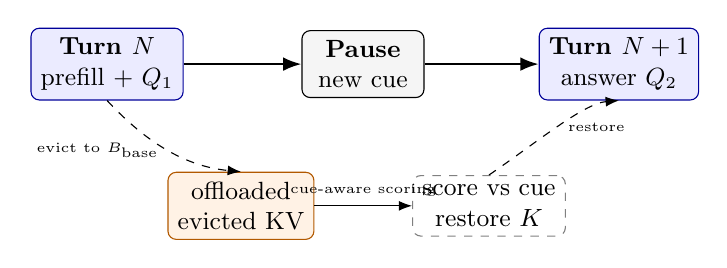
\begin{tikzpicture}[font=\small, >=Latex,
  box/.style={draw, rounded corners=3pt, align=center,
              inner sep=3.5pt, minimum width=1.55cm},
  gpu/.style={box, fill=blue!8, draw=blue!60!black},
  host/.style={box, fill=orange!10, draw=orange!70!black}]
  \node[gpu] (turnn) at (0,0) {\textbf{Turn $N$}\\prefill + $Q_1$};
  \node[box, fill=gray!8] (idle) at (3.25,0) {\textbf{Pause}\\new cue};
  \node[gpu] (turnn1) at (6.5,0) {\textbf{Turn $N+1$}\\answer $Q_2$};

  \node[host] (buf) at (1.7,-1.8) {offloaded\\evicted KV};
  \node[box, draw=gray, dashed] (score) at (4.85,-1.8) {score vs cue\\restore $K$};

  \draw[->, thick] (turnn) -- (idle);
  \draw[->, thick] (idle) -- (turnn1);
  \draw[->, dashed] (turnn.south) .. controls (0.5,-1.0) and (1.0,-1.3) .. (buf.north)
    node[midway, left, font=\tiny]{evict to $\bbase$};
  \draw[->] (buf.east) -- (score.west)
    node[midway, above, font=\tiny]{cue-aware scoring};
  \draw[->, dashed] (score.north) .. controls (5.45,-1.0) and (6.05,-0.5) .. (turnn1.south)
    node[midway, right, font=\tiny]{restore};
\end{tikzpicture}
\caption{\idlekv{} treats a paused compressed cache as repairable state.
Evicted KV rows are retained off-device, rescored once the next-turn cue
arrives, and selectively restored before resumed decoding.}
\label{fig:pipeline}
\end{figure}

\paragraph{Scoring.}
The main experiments use an exact $Q_2$ attention-query scorer.
After the $Q_2$ prompt is available, the prototype extracts the model's
$Q_2$ self-attention query vectors and scores evicted keys under
competition with active keys.
This scorer is useful as mechanistic evidence because it directly tests
whether the future cue identifies rows that the compressed cache omitted.
It is not claimed to be the final deployable scorer.
We also evaluate a cheaper proxy that appends $Q_2$ to the compressed
state and uses the resulting cache rows as scoring features.

\paragraph{Restore unit.}
\idlekv{} restores local bursts around high-scoring anchors rather than
isolated tokens.
This reflects the structure of retrieval-style contexts: the token that
matches a query key may be near, but not identical to, the value tokens
needed for the answer.
The restore budget $K$ counts restored context tokens after overlap
resolution.
It is not an anchor count, a byte budget, or an increase in preserved
prompt/answer-tail state.

\paragraph{Hindsight reference.}
We include $\goldk{}$ as a benchmark-metadata hindsight reference.
It selects from annotated $Q_2$ span groups using knowledge unavailable
to the runtime.
It is therefore not a deployable baseline and not a mathematical upper
bound over all token subsets.
Its role is to show how much headroom remains for better selectors under
the same restore budget.

% -----------------------------------------------------------------------
\section{Evaluation Protocol}
\label{sec:protocol}
% -----------------------------------------------------------------------

\paragraph{Task and model.}
The main diagnostic is split-query MQ-NIAH, a controlled relevance-shift
variant of multi-query needle-in-a-haystack derived from
RULER~\citep{ruler}.
Each example places key/value needles in a long distractor context.
$Q_1$ asks for one subset of values, the cache is compressed, and $Q_2$
asks for a different subset after the pause.
The main draft evaluation uses Qwen2.5-7B-Instruct at 32K context with a
context-only SnapKV first-stage compressor~\citep{qwen,snapkv}.

\paragraph{Conditions.}
All conditions reuse the same full-cache-generated $Q_1$ transcript
within a setting.
We compare full cache, base compressed cache, matched no-repair
$\bmatch$, Random-$K$, Oldest-$K$, \idlekv{}, and $\goldk{}$.
Random-$K$ and Oldest-$K$ restore from the same offloaded evicted-KV
store as \idlekv{} but ignore the $Q_2$ cue.
These controls test whether any benefit comes from cue-conditioned
selection rather than from generic reinsertion.

\paragraph{Specificity controls.}
The outline's central causal check is whether the next-turn cue matters.
We therefore compare true-$Q_2$ repair to stale-cue and donor-cue
repairs at a fixed operating point.
The stale cue reuses an earlier relevance signal; the donor cue comes
from another example.
If these controls match \idlekv{}, the method is only recovering generic
lost recency or needle structure.
If they stay near matched no-repair while \idlekv{} improves, the result
supports cue-specific repair.

\paragraph{Metrics.}
The main metric is exact $Q_2$ answer score: the fraction of requested
values recovered correctly, averaged over the fixed evaluation set.
For effect size, we report score gain over matched no-repair,
\begin{equation}
  \drepair =
  \mathrm{Score}(\mathrm{\idlekv}) - \mathrm{Score}(\bmatch).
\end{equation}
We also report overlap with annotated $Q_2$ spans, proxy/exact latency
tradeoffs, and per-partition endpoint checks.

% -----------------------------------------------------------------------
\section{Results}
\label{sec:results}
% -----------------------------------------------------------------------

\paragraph{Matched-budget frontier.}
Figure~\ref{fig:main-frontier} gives the primary quality result.
Across split-query MQ-NIAH query counts, \idlekv{} improves the resumed
$Q_2$ score over matched no-repair at the same active cache budget.
The gains are largest in stale-but-recoverable regimes: the base cache
has discarded useful future-query context, but the offloaded store still
contains rows that can be restored.
Random-$K$ and Oldest-$K$ remain near matched no-repair, indicating that
the effect is not explained by arbitrary extra tokens from the store.

\begin{figure}[t]
  \centering
  
\includegraphics[width=\columnwidth]{frontier_raw_overlay.pdf}
  \caption{Raw exact $Q_2$ score under matched resumed active-cache
  budgets. Solid curves show \idlekv{} and dotted curves show matched
  no-repair at the same resumed active KV budget.}
  \label{fig:main-frontier}
\end{figure}

\paragraph{Cue specificity.}
Figure~\ref{fig:specificity-control} checks whether repair depends on
the newly revealed $Q_2$ cue.
At the selected operating point, stale-cue and donor-cue repairs remain
near matched no-repair, while true-$Q_2$ \idlekv{} repair improves
substantially.
The same panel includes a stronger refresh-buffered comparator that
reselects the resumed active budget from active plus offloaded rows
using the $Q_2$ scores.
Refresh-buffered demonstrates remaining selector headroom; \idlekv{} is
an incremental repair primitive, not the strongest possible
store-backed post-$Q_2$ selector.

\begin{figure}[t]
  \centering
  
\includegraphics[width=\columnwidth]{specificity_control_dotplot.pdf}
  \caption{Next-turn cue specificity. True-$Q_2$ \idlekv{} repair gains
  over matched no-repair, while stale and donor cues remain near zero
  gain. Refresh-buffered is a stronger store-backed reselection
  comparator.}
  \label{fig:specificity-control}
\end{figure}

\paragraph{Operating regime.}
Repair is not uniformly useful.
When the active budget is too small, the restored budget may be
insufficient to recover enough context.
When the task is already saturated, there is little remaining headroom.
Figure~\ref{fig:operating-regime} maps the middle regime by plotting the
fraction of available $\goldk{}$ headroom recovered by \idlekv{} across
base and restore budgets.
This view is a calibration diagnostic rather than a cross-task effect
size: it shows where the current selector converts benchmark-specific
headroom into answer quality.

\begin{figure}[t]
  \centering
  
\includegraphics[width=\columnwidth]{operating_regime_heatmap.pdf}
  \caption{Operating-regime diagnostic. Cells report the fraction of
  available $\goldk{}$ headroom recovered by \idlekv{} under matched
  active-cache budgets.}
  \label{fig:operating-regime}
\end{figure}

\paragraph{Robustness and mechanism.}
Per-partition endpoint checks show that the high-$K$ result is not
carried by one favorable split.
The mechanism diagnostic is consistent with the quality result:
\idlekv{} moves the final active cache toward annotated $Q_2$ answer
spans, while matched no-repair and content-agnostic restores remain
close to their starting overlap.
Appendix checks with an H$_2$O-style first-stage compressor and a
preliminary Llama-3.1-8B-Instruct replication point in the same
direction, but they should be read as breadth checks rather than broad
model- or compressor-robustness claims.

\paragraph{Cost.}
The offloaded-store design changes the resource accounting.
The active device-resident cache is matched to $\bmatch$ at resumed
decode time, but \idlekv{} retains extra host-memory state and spends
time scoring and reinjecting selected rows.
Transfer and reinjection alone are modest in the current prototype, but
the exact $Q_2$ scorer is slow because it directly scores the evicted
pool.
The proxy scorer substantially reduces latency while preserving a
positive gain over matched no-repair in paired probes.
The current quality curves should therefore be read as evidence that
post-compression repair can work, while deployable repair needs faster
approximate scoring.

% -----------------------------------------------------------------------
\section{Discussion and Limitations}
\label{sec:discussion}
% -----------------------------------------------------------------------

\idlekv{} is not a replacement for KV compression, offload, or
query-aware access.
It is a between-turn maintenance primitive that becomes relevant when
the next turn supplies information unavailable at compression time.
The method should help when three conditions hold: the new turn changes
which old context matters, the compressed cache still has meaningful
choice among evicted rows, and the system has enough pause-window budget
or scheduling slack to perform repair.

The present evidence is intentionally controlled.
The task is synthetic retrieval, the next-turn cue is explicit, the main
model and compressor are fixed, and the exact scorer is not latency
competitive.
The matched-budget framing also matches only active GPU KV at resumed
decode time; it does not make the offloaded store free.
These constraints are part of the contribution rather than an accident:
they separate the core question of active-memory repair from broader
deployment questions that require additional workloads and systems
engineering.

Future work should evaluate realistic agent and tool-use workflows,
learn or approximate better selectors, account for byte-level and
latency-level budgets, and test architectures with different KV layouts.
The benchmark should also move beyond a single two-turn query split to
study conflicts, topic shifts, repeated revisions, and multi-turn
accumulation.

% -----------------------------------------------------------------------
\section{Conclusion}
\label{sec:conclusion}
% -----------------------------------------------------------------------

KV compression should not always be treated as a final memory decision.
In multi-turn workflows, later cues can reveal that the active cache is
stale before the next decode begins.
\idlekv{} shows that a paused compressed cache can be repaired by
restoring cue-relevant evicted KV under a matched resumed active-cache
budget.
The broader direction is mutable KV memory for resource-adaptive
long-context inference.

\begin{thebibliography}{13}

\bibitem[Abhyankar et~al.(2024)]{infercept}
Abhyankar, R., He, Z., Srivatsa, V., Zhang, H., and Zhang, Y.
\newblock InferCept: Efficient intercept support for augmented large
  language model inference.
\newblock In \emph{Proceedings of the 41st International Conference on
  Machine Learning (ICML)}, 2024.

\bibitem[Hsieh et~al.(2024)]{ruler}
Hsieh, C.-Y., Sun, S., Kriman, S., Acharya, S., Rekesh, D., Jia, F.,
  Zhang, Y., and Ginsburg, B.
\newblock RULER: What's the real context window size of your LLM?
\newblock \emph{arXiv:2404.06654}, 2024.

\bibitem[Kwon et~al.(2023)]{vllm}
Kwon, W., Li, Z., Zhuang, S., Sheng, Y., Zheng, L., Yu, C. H.,
  Gonzalez, J. E., Zhang, H., and Stoica, I.
\newblock Efficient memory management for large language model serving
  with PagedAttention.
\newblock In \emph{Proceedings of the 29th ACM Symposium on Operating
  Systems Principles (SOSP)}, 2023.

\bibitem[Li et~al.(2024)]{snapkv}
Li, Y., Huang, Y., Yang, B., Venkitesh, B., Locatelli, A., Ye, H.,
  Cai, T., Lewis, P., and Chen, D.
\newblock SnapKV: LLM knows what you are looking for before generation.
\newblock \emph{arXiv:2404.14469}, 2024.

\bibitem[Li et~al.(2025)]{scbench}
Li, Y., Jiang, H., Wu, Q., Luo, X., Ahn, S., Zhang, C., Abdi, A. H.,
  Li, D., Gao, J., Yang, Y., and Qiu, L.
\newblock SCBench: A KV cache-centric analysis of long-context methods.
\newblock In \emph{International Conference on Learning Representations
  (ICLR)}, 2025.

\bibitem[Chen et~al.(2025)]{pitfalls}
Chen, A., Geh, R., Grover, A., Van den Broeck, G., and Israel, D.
\newblock The pitfalls of KV cache compression.
\newblock \emph{arXiv:2510.00231}, 2025.

\bibitem[Qwen(2024)]{qwen}
Qwen Team.
\newblock Qwen2.5 technical report.
\newblock \emph{arXiv:2412.15115}, 2024.

\bibitem[Tang et~al.(2024)]{quest}
Tang, J., Zhao, Y., Zhu, K., Xiao, G., Kasikci, B., and Han, S.
\newblock QUEST: Query-aware sparsity for efficient long-context LLM
  inference.
\newblock In \emph{Proceedings of the 41st International Conference on
  Machine Learning (ICML)}, 2024.

\bibitem[Sun et~al.(2025)]{shadowkv}
Sun, H., Chang, L.-W., Bao, W., Zheng, S., Zheng, N., Liu, X., Dong,
  H., Chi, Y., and Chen, B.
\newblock ShadowKV: KV cache in shadows for high-throughput long-context
  LLM inference.
\newblock \emph{arXiv:2410.21465}, 2025.

\bibitem[Xiao et~al.(2024)]{streamingllm}
Xiao, G., Tang, Y., Zuo, J., Guo, J., Yang, S., Tang, H., Fu, Y.,
  and Han, S.
\newblock Efficient streaming language models with attention sinks.
\newblock In \emph{International Conference on Learning Representations
  (ICLR)}, 2024.

\bibitem[Zhang et~al.(2023)]{h2o}
Zhang, Z., Sheng, Y., Zhou, T., Chen, T., Zheng, L., Cai, R., Song, Z.,
  Tian, Y., R{\'e}, C., Barrett, C., Wang, Z., and Chen, B.
\newblock H$_2$O: Heavy-hitter oracle for efficient generative inference
  of large language models.
\newblock In \emph{Advances in Neural Information Processing Systems
  (NeurIPS)}, 2023.

\bibitem[Cai et~al.(2024)]{pyramidkv}
Cai, Z., Zhang, Y., Gao, B., Liu, Y., Liu, T., Lu, K., Xiong, W.,
  Dong, Y., Chang, B., Hu, J., and Xiao, W.
\newblock PyramidKV: Dynamic KV cache compression based on pyramidal
  information funneling.
\newblock \emph{arXiv:2406.02069}, 2024.

\end{thebibliography}

\appendix

\section{Appendix Draft Notes}
\label{app:draft-notes}

The appendix should make the controlled result auditable without
carrying the main claim.
Planned material includes prompt details, split definitions, the
$\goldk{}$ construction and caveats, per-partition endpoint plots,
selection-overlap diagnostics, H$_2$O-style compressor breadth,
preliminary model-transfer checks, and proxy/runtime accounting.
The final version should keep graph-first supplementary views and avoid
wide tables unless exact endpoint values are needed for reproducibility.

\section{Protocol Details To Fill}
\label{app:protocol-details}

The current draft should be extended with the final prompt text, decode
budgets, partition list, bootstrap procedure for confidence intervals,
and exact definitions of stale-cue, donor-cue, and refresh-buffered
controls.
These details are not needed to understand the main argument, but they
are important for auditability and should appear before submission.

\end{document}
